%\section{Extensions of \trip}

\subsection{Personalized Constraints}
\label{sec:personalized}

We next extend the basic MILP problem, outlined in Eq.~\eqref{eq:max}--Eq.~\eqref{eq:subtour} to incorporate personalized constraints.

\subsubsection{\textbf{Must-visit POIs}}
\label{sec:must}

Suppose the traveler specifies a list of POIs $[m_1, \dots, m_k]$ that she
must visit.  Simply enforcing the corresponding $y$ binary variables to
$1$ ensures that these POIs are chosen in the optimal itinerary:
%
\begin{align}
	\label{eq:see}
	y_{m_i} & = 1, \forall i = 1, \dots, k
\end{align}

\subsubsection{\textbf{Must-avoid POIs}}
\label{sec:avoid}

Similarly, if the traveler explicitly lists a set of POIs $[v_1, \dots,
v_k]$ that she does not want to visit, the corresponding $y$ binary
variables are simply set to $0$:
%
\begin{align}
	\label{eq:avoid}
	y_{a_i} & = 0, \forall i = 1, \dots, k
\end{align}

\subsubsection{\textbf{Category Constraints}}
\label{sec:category}

To handle category contraints where a traveler specifies the range of
number of POIs that she wants to visit for a category, we augment the
variable $y$ associated with every POI with a category superscript.  For
example, if there are $l$ categories, the corresponding variables $y^1,
\dots, y^l$ represent the different possibilities.  If POI $i$ belongs to
category $k$, then, by definition, $y^j_i = 0, \forall j \neq k$, for
every other category $j$.  If every category $k$ has a lower bound $lb^k$
and upper bound $ub^k$ on number of POIs to be visited, then the basic
problem can be augmented by:
%
\begin{align}
	\label{eq:category}
	lb^k \leq \sum_{i} y^k_i & \leq ub^k, \forall k
\end{align}
%
If the traveler only specifies the minimum number of POIs of a category
$k$ that she must visit, the upper bound $ub^k = N$; similarly, specifying
only the maximum number puts the lower bound as $lb^k = 0$.  For
categories where no constraint is mentioned, $lb^k = 0$ and $ub^k = N$, where N is the number of POIs of that category.

\subsubsection{\textbf{Ordering Constraints}}
\label{sec:ordering}

A traveler can impose an ordering constraint, where she will visit POI $j$ before POI $k$, if the itinerary contains both of them.
To impose these ordering constraints, we use the \emph{arrival time} of the POIs.
If POI $j$ must be visited before POI $k$ (denoted as $j \prec k$), then $a_k$ must be after $a_j$ plus
the time it takes to visit $v_j$ (i.e., $t_{v_j}$) and the time it takes to
reach $v_k$ from $v_j$ (i.e., $t_{j,k}$).
Hence,
%
\begin{align}
	a_j + t_{j} + t_{j,k} & \leq a_k, \forall j \prec k
\end{align}
%
The above equation assumes that both POIs $j$ and $k$ are visited.
However, it may be the case that $j$ or $k$ or both are not visited.
To handle the case that $j$ is not visited, the lower bound of $a_j$ for any
node is kept as $0$, and the times are added only if $y_j = 1$.
To handle the case that $k$ is not visited, a large value $M$ is added to $a_k$
when $y_k = 0$.
Together, the ordering constraint equation becomes
%
\begin{align}
	\label{eq:ordering}
	a_j + (t_{j} + t_{j,k}) \cdot y_j & \leq a_k + M \cdot (1 - y_k), \forall j \prec k
\end{align}

\subsection{POI Timings}
\label{sec:timings}

Many POIs have certain operating times.  For example, a temple may be open
only in the morning, from 9-11am.  Even otherwise, a traveler may specify that she wants to visit the temple in the morning hours only.  To handle this constraint, the start and
end time of the POI must be within this operational time.  Hence, if a POI
$i$ has an operational time denoted by entry and exit times $[en_i, ex_i]$,
then
%
\begin{align}
	\label{eq:operational}
	s_i \geq en_i \text{ and } & s_i + t_{i} \leq ex_i, \forall i
\end{align}

\subsection{Utility Variants}
\label{sec:utility}

The basic problem formulation assumes a traveler visits a POI for a fixed amount
of time, and gets the full utility offered by the POI.  However, in real life,
the time spent by every traveler is not the same.  Some may finish visiting a
POI in lesser time than the prescribed one, while some others may take longer
time.  In addition, some may not be willing to spend the full time in a POI, and
may sacrifice getting the full utility for partial utilization, and may come out
early to save time, and visit other POIs.  For example, a museum may have many
different types of rooms, such as sculpture, paintings, jewelry, etc., and a
traveler may not like to visit the jewelry section.  She may, thus, decide to
spend only a part of the total visit time for the other sections, get a partial
utility, and exit to go to another POI.  To capture this, we model the utility
in three variants, as described next.
Fig.~\ref{fig:utility} graphically shows the three variants.
Note that in all of these variants, if a traveler spends \emph{more} time
than the prescribed time of visit, her utility is capped to 100\% only.

\subsubsection{\textbf{Binary}}
\label{sec:binary}

This is the standard utlity variant, where a traveler spends full time in a
POI, and gets the complete utility.  If she does not spend that time, she
gets no utility at all.

The binary utility $U^b_i$ of a POI $i$ for the binary variant is captured
simply by
%
\begin{align}
	\label{eq:binary}
	U^b_i & = U_i, \forall i
\end{align}

\subsubsection{\textbf{Slab}}
\label{sec:slab}

The binary utility variant is too strict and does not allow any leeway.
In the slab utility variant, the total visit time is divided into various slabs, starting from
0.5.  (We assume that a POI must be visited for at least half of its prescribed time
to obtain any utility.) Each \emph{slab} is an interval of time spent as a percentage
of the total visit time.  When a traveler spends time in a slab of
interval, she gets a percentage of utility equal to the lower end of the
interval.  Thus, if a slab is $[0.6-0.7)$ and a traveler spends $0.67$ time,
she gets a utility equal to $0.6$ of the total utility.

The utility value is divided into the same number of slabs as the visit
time.  In this paper, we divide into 6 slabs: $[0.5-0.6), [0.6-0.7), [0.7-0.8),
[0.8-0.9), [0.9-1.0), [1.0-\infty)$, although this can be altered.
Consequently, we have six binary \emph{slab variables} for every POI,
$u^1, \dots, u^6$, with the constraint that at most one of them is chosen
(using the condition $\sum_{l=1}^6 u^l_i \leq 1$).  The \emph{effective
utility} of a POI $i$ is then:
%
\begin{align}
	\label{eq:slab}
	U^s_i = U_i \cdot ( & 0.5 \times u^1_i + 0.6 \times u^2_i + 0.7 \times u^3_i \nonumber \\
		& + 0.8 \times u^4_i + 0.9 \times u^5_i + 1.0 \times u^6_i )
\end{align}

\subsubsection{\textbf{Continuous}}
\label{sec:continuous}

The third variant models the utility as a continuous function equal to the
percentage of time spent.  (Again, we impose the minimum time to be spent
as 50\% for non-zero utility.) Thus, if a traveler spends 67\% time, she
gets 67\% utility.

The continuous variant introduces a variable $f_i \in (0,1)$ to denote the fraction of utility got from a POI, corresponding to the time spent there.
Its upper and lower bounds are set to 1.0 and 0.5 respectively in the following manner:
%
\begin{align}
	\label{eq:fbound1}
	f_i & \geq 0.5 \cdot y_i \\
	\label{eq:ybound1}
	y_i & \geq f_i - (0.5 - \epsilon) \\
    \label{eq:fbound2}
	f_i & \leq y_i \\
	\label{eq:ybound2}
    y_i & \leq f_i + (0.5 - \epsilon)
\end{align}
%
Eq.~\eqref{eq:fbound1} and Eq.~\eqref{eq:ybound1} ensure that if $y_i = 1$, i.e., if a POI is chosen, $f_i$ is at least $0.5$, and vice versa, i.e., if $f_i \geq 0.5$, then $y_i$ must be $1$. Eq.~\eqref{eq:fbound2} and
Eq.~\eqref{eq:ybound2} ensure the complementary condition, i.e., if $f_i
< 0.5$, then $y_i = 0$, and vice versa.  ($\epsilon$ is a
tiny positive constant.)

The utility $U^c_i$ is then simply the following.
%
\begin{align}
	\label{eq:continuous}
	U^c_i = U_i \cdot f_i
\end{align}

\begin{figure}[t]
\centering
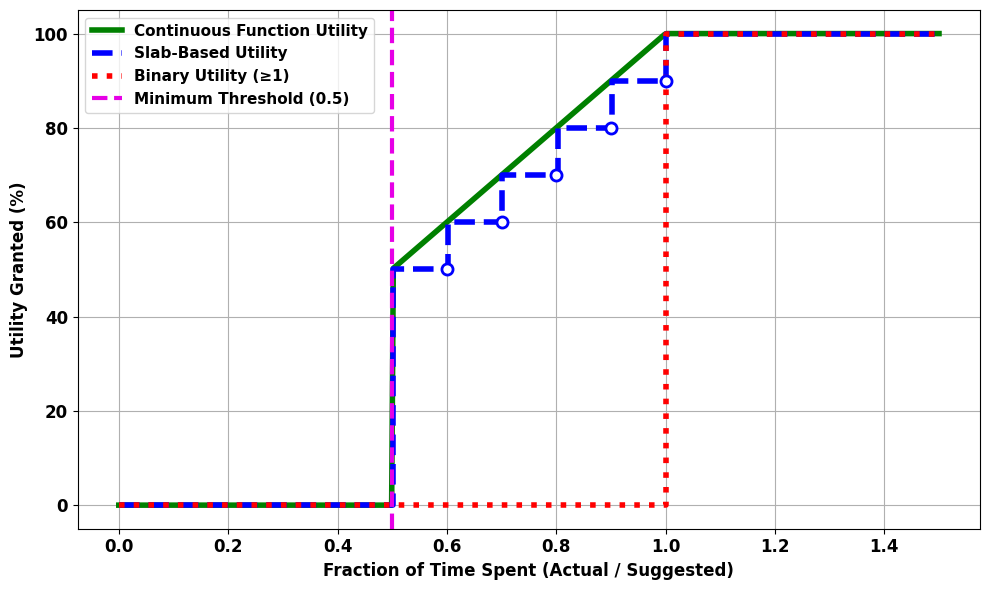
\includegraphics[width=\columnwidth]{plots/UF_Combined.png}
\figcaption{Different utility function variants}
\label{fig:utility}
\end{figure}

\subsection{Multi-Day Itinerary}
\label{sec:multiday}

For large tourist-friendly cities, covering all the POIs may not be
possible within a single day, and travelers typically look for
\emph{multi-day} tour itineraries.
Using a single-day solution, a multi-day itinerary can be simulated
by first
running for a single day, then getting rid of the POIs covered in that day, and
after that running again for the next day, and so on.
Instead, we solve the
problem as one single optimization problem.  For each day, we can specify a
source and destination, and the time budget.  This caters to tours where
the time in the first and last days are typically less due to arrival and
departure constraints.  Also, the first day's source and the last day's
destination may be an airport, while for other days, it
may be a hotel.

For an itinerary having $d$ days, we augment all the variables with a
superscript that indicates the day of the visit.  Thus, the $y$ and $z$
binary variables are replicated for each day: $y^d_i$ and $z^{m,d}_{j,k}$
for all POIs $i$, modes of transport $m$ and days of visit $d$.  While the
cost budget (Eq.~\eqref{eq:cost}) is imposed on the overall tour, the time
budget constraints (Eq.~\eqref{eq:time}) are imposed per day.  The rest of
the constraints (in Fig.~\ref{fig:basic})
remain the same, and are applied for each day.  Additionally, the following
conditions ensure that a POI is chosen at most once within $d$ days:
%
\begin{align}
	\label{eq:multiday}
	\sum_{\forall d} y^d_i & \leq 1, \forall i
\end{align}
%
Choosing a POI at most once automatically constraints choosing any incoming
or outgoing edge to or from it to at most once as well.

\subsection{Dynamic Itinerary Re-planning}
\label{sec:dynamic}

So far, we have discussed only static plans.
Once an optimal tour is decided, it is not altered.
However, in real life, both tourist behavior as well as other conditions including weather, traffic, etc. are not deterministic in nature, and change over time.
To handle this, we introduce \emph{dynamic tour re-planning} where we keep computing the best tour given the current situation.
To the best of our knowledge, no other tour planner does that.

We initially start with an optimal static plan using our solver that takes into account the traveler's preferences.
However, after visit of every POI, we provide an option to her to \emph{re-optimize} the rest of the plan based on the current situation.
This may happen since she may have spent substantially less or more time in a POI, or the current traffic condition has somehow altered significantly due to accidents, etc.
%
The \trip solver now re-plans the schedule based on the remaining time and cost
budgets. The POIs already visited are not considered further, and the current POI is considered the source.
This optimizes the rest of the tour based on current progress, which may be quite different from the initial
static setting.

